\documentclass[11pt,a4paper]{article}
\usepackage{fontspec}
\usepackage{xeCJK}
\setCJKmainfont{SimSun}
\setCJKsansfont{Microsoft YaHei}
\setCJKmonofont{SimSun}
\usepackage[margin=1.9cm]{geometry}
\usepackage{xcolor}
\usepackage{tikz}
\usetikzlibrary{arrows.meta,positioning,fit,calc}
\usepackage{booktabs}
\usepackage{tabularx}
\usepackage{array}
\usepackage{enumitem}
\usepackage{fancyhdr}
\usepackage{hyperref}
\usepackage{listings}

\definecolor{navy}{HTML}{17365D}
\definecolor{blue}{HTML}{2F75B5}
\definecolor{lightblue}{HTML}{EEF5FA}
\definecolor{green}{HTML}{548235}
\definecolor{lightgreen}{HTML}{EEF6EA}
\definecolor{orange}{HTML}{C55A11}
\definecolor{lightorange}{HTML}{FFF3E8}
\definecolor{gray}{HTML}{5B6573}
\hypersetup{colorlinks=true,linkcolor=blue,urlcolor=blue}
\setlength{\parindent}{0pt}
\setlength{\parskip}{4pt}
\setlist[itemize]{leftmargin=1.5em,itemsep=2pt,topsep=3pt}
\setlist[enumerate]{leftmargin=1.7em,itemsep=2pt,topsep=3pt}
\setlength{\emergencystretch}{3em}
\sloppy

\pagestyle{fancy}
\fancyhf{}
\setlength{\headheight}{14pt}
\fancyhead[L]{\textcolor{gray}{Tri-EvoBench | Baseline Integration}}
\fancyhead[R]{\textcolor{gray}{2026-08-28}}
\fancyfoot[C]{\textcolor{gray}{\thepage}}

\newenvironment{callout}{\begin{quote}\small\color{navy}}{\end{quote}}
\newcommand{\status}[2]{\textcolor{#1}{\textbf{#2}}}
\newcommand{\code}[1]{\texttt{#1}}

\title{\vspace{-1.2cm}\textcolor{navy}{Tri-EvoBench}\par\vspace{4pt}\Large Hermes、SkillOpt 与 Trace2Skill 的统一接入及真实评测状态}
\author{项目组}
\date{2026 年 8 月 28 日}

\begin{document}
\maketitle
\thispagestyle{empty}

\begin{center}
\textcolor{gray}{统一运行协议下的三个 baseline：接入方式、真实任务轨迹与当前成品状态}
\end{center}

\vspace{5pt}
\begin{callout}
Tri-EvoBench 当前已经不是单一 agent 的演示脚本，而是一层可以承载不同 agent 框架的评测运行时。Hermes、SkillOpt 和 Trace2Skill 都通过同一套 Flow/Turn/Interaction/Evolution 生命周期进入 Runner；差异保留在各自的 bridge 中，公共评测、公开轨迹、token 计量、状态快照和结果格式保持一致。
\end{callout}

\section{当前成品总览}

\begin{center}
\begin{tikzpicture}[node distance=8mm and 7mm, >=Latex, every node/.style={font=\small},
  core/.style={rounded corners=2pt, draw=navy, fill=lightblue, minimum height=14mm, text width=31mm, align=center},
  base/.style={rounded corners=2pt, draw=green!70!black, fill=lightgreen, minimum height=14mm, text width=30mm, align=center},
  result/.style={rounded corners=2pt, draw=orange!80!black, fill=lightorange, minimum height=14mm, text width=31mm, align=center}]
\node[core] (runner) {Tri-EvoBench Runner\\统一生命周期与预算};
\node[base, below left=of runner] (hermes) {Hermes\\Docker + SessionManager};
\node[base, below=of runner] (skillopt) {SkillOpt\\target + skill reflection};
\node[base, below right=of runner] (trace) {Trace2Skill\\tool trace + skill evolution};
\node[result, below=of skillopt, yshift=-12mm] (judge) {公开轨迹 + Judge\\summary / trace / snapshot};
\draw[->, thick, navy] (runner) -- (hermes);
\draw[->, thick, navy] (runner) -- (skillopt);
\draw[->, thick, navy] (runner) -- (trace);
\draw[->, thick, orange!80!black] (hermes) |- (judge);
\draw[->, thick, orange!80!black] (skillopt) -- (judge);
\draw[->, thick, orange!80!black] (trace) |- (judge);
\end{tikzpicture}
\end{center}

三个 baseline 的统一输入输出关系如下：

\begin{center}
\renewcommand{\arraystretch}{1.25}
\begin{tabularx}{0.98\linewidth}{>{\bfseries}p{0.22\linewidth}XXX}
\toprule
层次 & Hermes & SkillOpt & Trace2Skill \\
\midrule
运行入口 & Docker process adapter；复用 Hermes ACP SessionManager & 独立 NDJSON bridge；调用 target backend & 独立 NDJSON bridge；运行 CLIOnly/CLISkillPreloaded agent \\
工作区 & 共享 \code{/workspace}；状态挂载 \code{/hermes-state} & 共享 workspace；Flow 独占 \code{skill.md} 与 \code{history/} & 共享 workspace；Flow 独占 \code{skills/} 与 \code{history/} \\
学习阶段 & Hermes background/native review 或 barrier 记录 & Reflect -> Aggregate -> Clip -> Update & MAP -> REDUCE -> APPLY -> VERIFY \\
输出轨迹 & 回复、模拟工具、事件、状态更新、judge & 回复、\code{write\_file} action、skill hash、usage & 回复、真实 tool calls、步骤 trace、skill/evolution 文件 \\
\bottomrule
\end{tabularx}
\end{center}

\section{统一接入方式}

每个 baseline 都实现同一组生命周期方法。Runner 不需要理解某个框架内部的 session、skill 或工具实现，只消费 bridge 返回的结构化结果。

\begin{enumerate}
\item \textbf{initialize：} 校验 protocol version，声明 capabilities，并读取 manifest 中的环境与运行参数。
\item \textbf{start\_flow：} 创建 Flow 独占的状态目录和共享 workspace，装载初始 skill/memory，并返回状态快照信息。
\item \textbf{start\_turn：} 建立新会话；Turn 不继承聊天 history，但继续使用同一 Flow 的学习状态。
\item \textbf{interact：} 将一次 benchmark 请求翻译成框架原生调用，返回最终文本、公开 tool/action 轨迹、事件和增量 usage。
\item \textbf{evolve：} 只接收公开 trajectory 与公开 judge feedback；完成后才能进入下一 Turn。
\item \textbf{snapshot/end\_flow：} 对声明的学习状态做 hash 和 diff，导出 summary、trace、快照，清理临时配置与 session 数据库。
\end{enumerate}

\begin{callout}
关键隔离边界：\code{verifier\_details}、\code{oracle\_update}、私有 evaluator 文件和私有 metadata 不进入 baseline bridge。Judge 能看到的是公开任务、公开交互和允许检查的文件；因此不同 baseline 的分数在同一可见性边界下可比较。
\end{callout}

\section{Hermes：从上游 Session 到 Tri-EvoBench Flow}

Hermes 的接入保留上游能力，同时把外层生命周期交给 Tri-EvoBench：

\begin{itemize}
\item manifest 启动受限 Docker 容器，挂载共享 workspace 和 Flow 状态目录，并通过环境白名单透传模型凭据；
\item bridge 直接复用 Hermes 的 SessionManager、AIAgent、SessionDB 和工具集，不要求 Runner 理解 ACP；
\item L1 通过协议 action/event 记录副作用，L2 保留 native private verifier 边界；
\item 每个 Turn 结束后进入 evolution barrier，Runner 记录学习状态变化与 token usage。
\end{itemize}

\subsection*{真实 Hermes L1 运行：一个 Turn 的完整闭环}

在 \code{runs/merge-hermes-l1-full-final/} 的 7-turn 真实运行中，第一轮展示了澄清、重试和工具调用如何串起来：

\begin{center}
\begin{tikzpicture}[node distance=5mm and 4mm, >=Latex, every node/.style={font=\scriptsize},
  b/.style={rounded corners=2pt, draw=blue!75!black, fill=lightblue, minimum height=12mm, text width=31mm, align=center},
  g/.style={rounded corners=2pt, draw=green!70!black, fill=lightgreen, minimum height=12mm, text width=31mm, align=center}]
\node[b] (r1) {Turn 1 / interaction 1\\识别缺少 calendar id};
\node[b, right=of r1] (u) {用户澄清\\cal\_delivery\_team};
\node[g, right=of u] (r2) {interaction 2\\calendar.create\_event};
\node[g, right=of r2] (j) {Judge\\score 0.95 / pass};
\draw[->, thick, navy] (r1) -- (u);
\draw[->, thick, navy] (u) -- (r2);
\draw[->, thick, navy] (r2) -- (j);
\end{tikzpicture}
\end{center}

第一轮的可观察字段为：

\begin{itemize}
\item 初次回复触发 \code{asked\_for\_calendar\_id}，没有在不确定时直接创建事件；
\item 澄清后调用 \code{calendar.create\_event}，参数包含 \code{calendar\_id=cal\_delivery\_team}、标题 \code{Aurora 周例会}、时间 \code{2026-08-24 10:00-10:30 +08:00}；
\item Judge 对任务完成、工具参数、记忆事实和回复语言分别评分，最终 0.95，唯一扣分是澄清事实没有在创建前以可观察状态再次记录。
\end{itemize}

同一运行的后续真实经历包括：Turn 2 首次未执行文件和群组动作，重试后产生风险清单文件并修正群组 ID；Turn 5 首次未写入润色文件，重试后生成 \code{docs/abstract\_polished.txt}；Turn 6 生成中文摘要文件。最终 7 turns、13 interactions，平均分 0.9214，turn 通过率 100\%。这说明 Hermes 接入已经能把“失败 -> feedback -> retry -> action -> judge”完整保留下来。

\subsection*{Hermes 长流压力结果}

GLM-5.3-Flash 下的两条 60-turn L1-Life v2 流进一步验证了长流成品：

\begin{center}
\renewcommand{\arraystretch}{1.25}
\begin{tabular}{lrrrrr}
\toprule
流 & turns & interactions & API calls & 平均分 & 严格通过率 \\
\midrule
stream-1 & 60 & 62 & 131 & 0.1363 & 0\% \\
stream-2 & 60 & 62 & 139 & 0.1524 & 0\% \\
合计 & 120 & 124 & 270 & 0.1444 & 0\% \\
\bottomrule
\end{tabular}
\end{center}

所有 turns 均落盘且 judge 请求无 HTTP 错误；低分来自 iteration limit、未触发记忆激活和未完成结构化任务。该长流结果与上面的 7-turn 成功链路共同说明：运行时接入和审计链路已稳定，长期任务完成能力仍是独立的模型问题。

\section{SkillOpt：把 target agent 与 skill 更新接入同一 Flow}

SkillOpt bridge 的职责是把 Tri-EvoBench 的 Interaction 请求交给 target backend，把公开反馈交给 skill 优化流程，并把学习状态限制在 Flow 目录：

\begin{center}
\begin{tikzpicture}[node distance=8mm and 5mm, >=Latex, every node/.style={font=\small},
  b/.style={rounded corners=2pt, draw=blue!75!black, fill=lightblue, minimum height=12mm, text width=32mm, align=center},
  g/.style={rounded corners=2pt, draw=green!70!black, fill=lightgreen, minimum height=12mm, text width=32mm, align=center}]
\node[b] (req) {Runner request\\+ 当前 skill.md};
\node[b, right=of req] (target) {SkillOpt target\\chat / exec};
\node[g, right=of target] (action) {公开结果\\write\_file / response};
\node[g, below=of action] (evo) {Reflect -> Aggregate\\Clip -> Update};
\draw[->, thick, navy] (req) -- (target);
\draw[->, thick, navy] (target) -- (action);
\draw[->, thick, orange!80!black] (action) -- (evo);
\draw[->, thick, orange!80!black] (evo) -| (req.south);
\end{tikzpicture}
\end{center}

真实运行 \code{runs/merge-skillopt-real/deepseek-flow-001/} 共 5 turns、5 interactions，平均分和通过率均为 1.0。五个任务覆盖了 SkillOpt 的核心闭环：

\begin{center}
\renewcommand{\arraystretch}{1.2}
\begin{tabularx}{0.98\linewidth}{lXll}
\toprule
任务 & 真实请求与可观察产物 & 动作/工具 & 结果 \\
\midrule
profile-fact & 创建 \code{/workspace/profile.txt}，写入 name=Lin、language=Chinese & \code{write\_file} & 1.0 \\
delayed-use & 读取 profile fact，再创建 \code{greeting.txt} & \code{write\_file} & 1.0 \\
config-repair & 将 \code{mode=development} 改为 production，保留其他键 & \code{write\_file} & 1.0 \\
json-artifact & 生成 status/owner/items 的有效 JSON & \code{write\_file} & 1.0 \\
llm-judge & 一句话总结 owner Lin、status ready、two items & 纯文本 & 1.0 \\
\bottomrule
\end{tabularx}
\end{center}

这里的关键不是把 SkillOpt 改造成 Runner，而是把它的 target 行为和 skill 更新阶段分别映射到 \code{interact} 与 \code{evolve}；Runtime 同时冻结 Interaction 期间的学习文件，防止未经 barrier 的持久写入。

\section{Trace2Skill：把工具轨迹变成可演化 Skill}

Trace2Skill bridge 保留原生工具使用方式，但把步骤转换成公共 trace，并在 Turn 边界执行演化：

\begin{center}
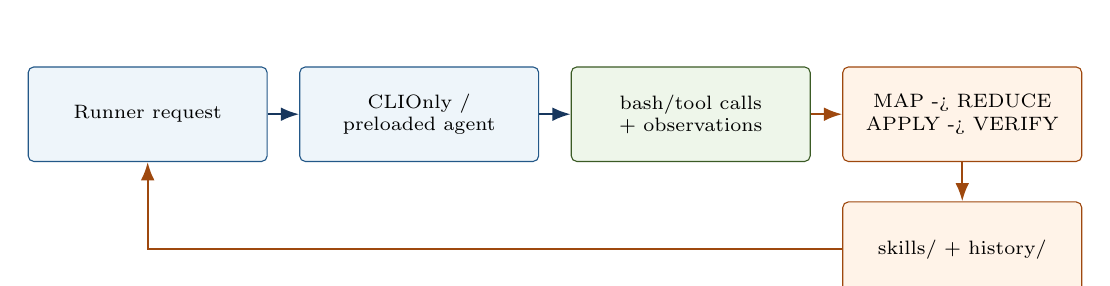
\begin{tikzpicture}[node distance=5mm and 4mm, >=Latex, every node/.style={font=\scriptsize},
  b/.style={rounded corners=2pt, draw=blue!75!black, fill=lightblue, minimum height=12mm, text width=28mm, align=center},
  g/.style={rounded corners=2pt, draw=green!70!black, fill=lightgreen, minimum height=12mm, text width=28mm, align=center},
  o/.style={rounded corners=2pt, draw=orange!80!black, fill=lightorange, minimum height=12mm, text width=28mm, align=center}]
\node[b] (r) {Runner request};
\node[b, right=of r] (a) {CLIOnly / preloaded agent};
\node[g, right=of a] (t) {bash/tool calls\\+ observations};
\node[o, right=of t] (e) {MAP -> REDUCE\\APPLY -> VERIFY};
\node[o, below=of e] (s) {skills/ + history/};
\draw[->, thick, navy] (r) -- (a);
\draw[->, thick, navy] (a) -- (t);
\draw[->, thick, orange!80!black] (t) -- (e);
\draw[->, thick, orange!80!black] (e) -- (s);
\draw[->, thick, orange!80!black] (s) -| (r.south);
\end{tikzpicture}
\end{center}

修复后的真实运行 \code{runs/merge-trace2skill-real-fixed/deepseek-flow-001/} 为 5 turns、6 interactions，平均分和通过率均为 1.0，首交互通过率 0.8。可观察的典型经历是 delayed-use：agent 第一次错误地把 Windows 临时路径当作容器路径，随后通过 \code{pwd}、\code{ls}、\code{cat} 发现共享 workspace 中的 profile，创建并验证 \code{greeting.txt}，最终任务通过。该运行同时在状态目录留下每个 Turn 的 \code{trajectory.json}、\code{feedback.json}、\code{evolution.json} 和 skill patch，说明工具轨迹确实进入了 skill 演化链。

\section{三者合在一起后的成品状态}

\begin{center}
\renewcommand{\arraystretch}{1.3}
\begin{tabularx}{0.98\linewidth}{>{\bfseries}p{0.25\linewidth}X}
\toprule
评测维度 & 当前成品证据 \\
\midrule
统一可替换性 & 通过 manifest 选择 baseline；Runner 生命周期不随 Hermes、SkillOpt、Trace2Skill 改写。 \\
真实副作用 & Hermes L1 与 SkillOpt 产生可验证文件/事件；Trace2Skill 产生真实终端观察与文件结果。 \\
跨回合学习 & Hermes 保留 memory/skills；SkillOpt 保留 skill.md/history；Trace2Skill 保留 skills/history，并在 barrier 后演化。 \\
可审计性 & 每个 Flow 有 summary、trace、usage、状态快照；judge 只消费公开证据。 \\
当前短板 & 短流任务已能稳定通过；GLM 长流的 iteration limit、记忆激活和结构化状态更新仍导致 L1-Life 严格通过率为 0\%。 \\
\bottomrule
\end{tabularx}
\end{center}

Hermes L2 还保留了一条独立的 native runtime 证据：\code{runs/merge-hermes-l2-real/} 中的 BigCodeBench Pandas 可视化 Episode E001/E002 均通过 private verifier，演化记录为 \code{evolution.completed}。这与 L1 的公开 judge 轨迹是两种不同层级的验证，但都已经进入统一的 Flow/episode 结果目录。

\section{结论}

Tri-EvoBench 的当前成品是一个可以承载不同 agent 框架的统一评测层：

\begin{itemize}
\item Hermes 证明了 Docker、SessionManager、memory/skills 和 L1/L2 verifier 可以被纳入统一生命周期；
\item SkillOpt 证明了 target agent 与 Reflect/Aggregate/Clip/Update skill 学习可以在 Flow 边界内运行；
\item Trace2Skill 证明了真实工具轨迹可以被转换为公开 evidence，并进入 MAP/REDUCE/APPLY/VERIFY 技能演化；
\item 三者都输出相同语义的 Flow/Turn/Interaction/Evolution 结果，允许后续做跨 baseline 比较；
\item 目前需要继续优化的是 agent 在长流中的任务完成、记忆激活和结构化动作，而不是再重做 baseline 接入层。
\end{itemize}

\end{document}
